\section{Alternative meshes with Gmsh}
\label{app:gmsh_meshes}

During the development of the spatial models, Gmsh was investigated as an alternative to the structured meshes used in the final implementation. Gmsh allows more flexible geometries and local control of the element size, for example by refining the mesh close to boundaries or other regions where large solution gradients are expected \cite{gmsh_manual,geuzaine2009gmsh}.

Two example battery geometries were created during this investigation. The first example, shown in Figure~\ref{fig:app_gmsh_2d}, demonstrates how the metal-hydride domain can be represented using a non-uniform two-dimensional mesh. Local mesh refinement can be introduced close to the hydrogen inlet, where the largest pressure and density gradients are expected during the initial filling stage. In addition to the metal-hydride domain, a surrounding region is included that could represent a temperature-regulating material. Possible examples are a cooling or heating medium or a phase-change material such as the PCM jacket considered by Darzi et al. The separate domains could then be assigned different material properties and coupled through their common interface. Using gmsh to create meshes can also make defining different boundaries and inlets easier, since you can give nodes a keyword upon creation.

\begin{figure}[ht]
\centering
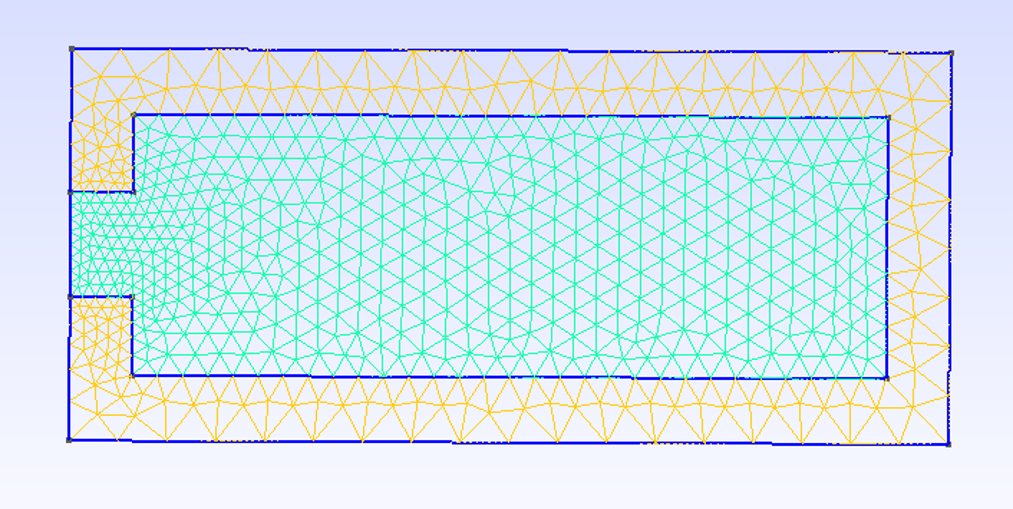
\includegraphics[width=0.8\textwidth]{figures/app_gmsh_2d.png}
\caption{Example of a two-dimensional mesh generated with Gmsh. The green region represents the metal-hydride domain in which hydrogen mass transfer takes place. The mesh can be refined locally, for example near the hydrogen inlet.}
\label{fig:app_gmsh_2d}
\end{figure}

A second example is shown in Figure~\ref{fig:app_gmsh_3d}. This example demonstrates how a three-dimensional battery geometry can be represented using a non-uniform mesh in Gmsh. Similar to the two-dimensional case, local mesh refinement can be applied near the hydrogen inlet or other regions with expected large solution gradients. The surrounding temperature-regulating material is also included and can be assigned different material properties from the metal-hydride bed.

\begin{figure}[ht]
\centering
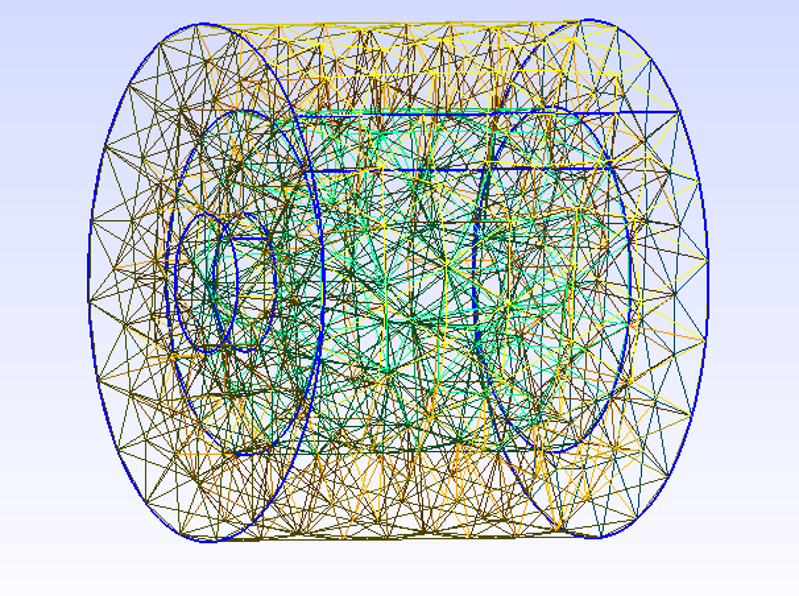
\includegraphics[width=0.8\textwidth]{figures/app_gmsh_3d.png}
\caption{Example of a three-dimensional battery geometry and mesh generated with Gmsh. The green region represents the metal-hydride bed, while the yellow region represents a possible surrounding temperature-regulating material, such as a coolant region or phase-change material.}
\label{fig:app_gmsh_3d}
\end{figure}

This approach was not pursued further in the present work. The priority was first to establish and validate the governing equations, finite-element discretization, mass-transfer implementation, and time integration on simpler structured meshes. Introducing more complex geometries at the same stage would have made it more difficult to distinguish errors in the physical and numerical formulation from errors related to mesh generation or domain coupling.

The Gmsh meshes may nevertheless become useful in future extensions of the model. This is particularly relevant if temperature is included. A surrounding thermal domain could then be modelled explicitly and coupled to the metal-hydride bed through heat conduction. Local mesh refinement could also be used near the hydrogen inlet, material interfaces, or cooled boundaries where stronger spatial gradients may occur. Gmsh therefore provides a possible route towards more realistic battery geometries once the thermal formulation has been established.
